\section{Risultati sperimentali}

\subsection{Simulazioni}
Il funzionamento del componente è stato verificato tramite l'utilizzo di appositi test bench. Sono state eseguite due tipi di simulazioni: \textit{Behavioural} e \textit{Post-Synthesis Functional}.\newline
Oltre al test bench di esempio sono stati creati altri test bench che cercassero di testare i vari scenari e casi limite di esecuzione del modulo. Le situazioni che sono state controllate sono le seguenti:
\begin{enumerate}
	\item \textbf{Caso base}: sequenza con valori vari, tra cui quelli forniti nelle specifiche.
        \item \textbf{Tutte parole valide}: sequenza in cui tutte le parole sono valide, quindi a tutte è associata la massima credibilità.
        \item \textbf{Credibilità fino a 0}: sequenza in cui solo la prima parola è valida, quindi si controlla il corretto decremento della credibilità da 31 a 0.
        \item \textbf{Prima parola 0}: sequenza in cui la prima parola è zero, quindi relativa credibilità zero.
        \item \textbf{Tutti 0}: sequenza di tutti zero, in cui la credibilità è ovunque nulla.
        \item \textbf{Reset durante un elaborazione}: il reset interrompe l'esecuzione della prima sequenza, a cui segue l'inizio di una successiva elaborazione.
        \item \textbf{Doppio start senza reset}: elaborazione di due sequenze senza ricevere il reset.
\end{enumerate}

\subsection{Sintesi}
Il componente è stato sintetizzato con successo. Riportiamo di seguito i risultati ottenuti dallo strumento di sviluppo Vivado.
\begin{figure}[H]
    \centering
    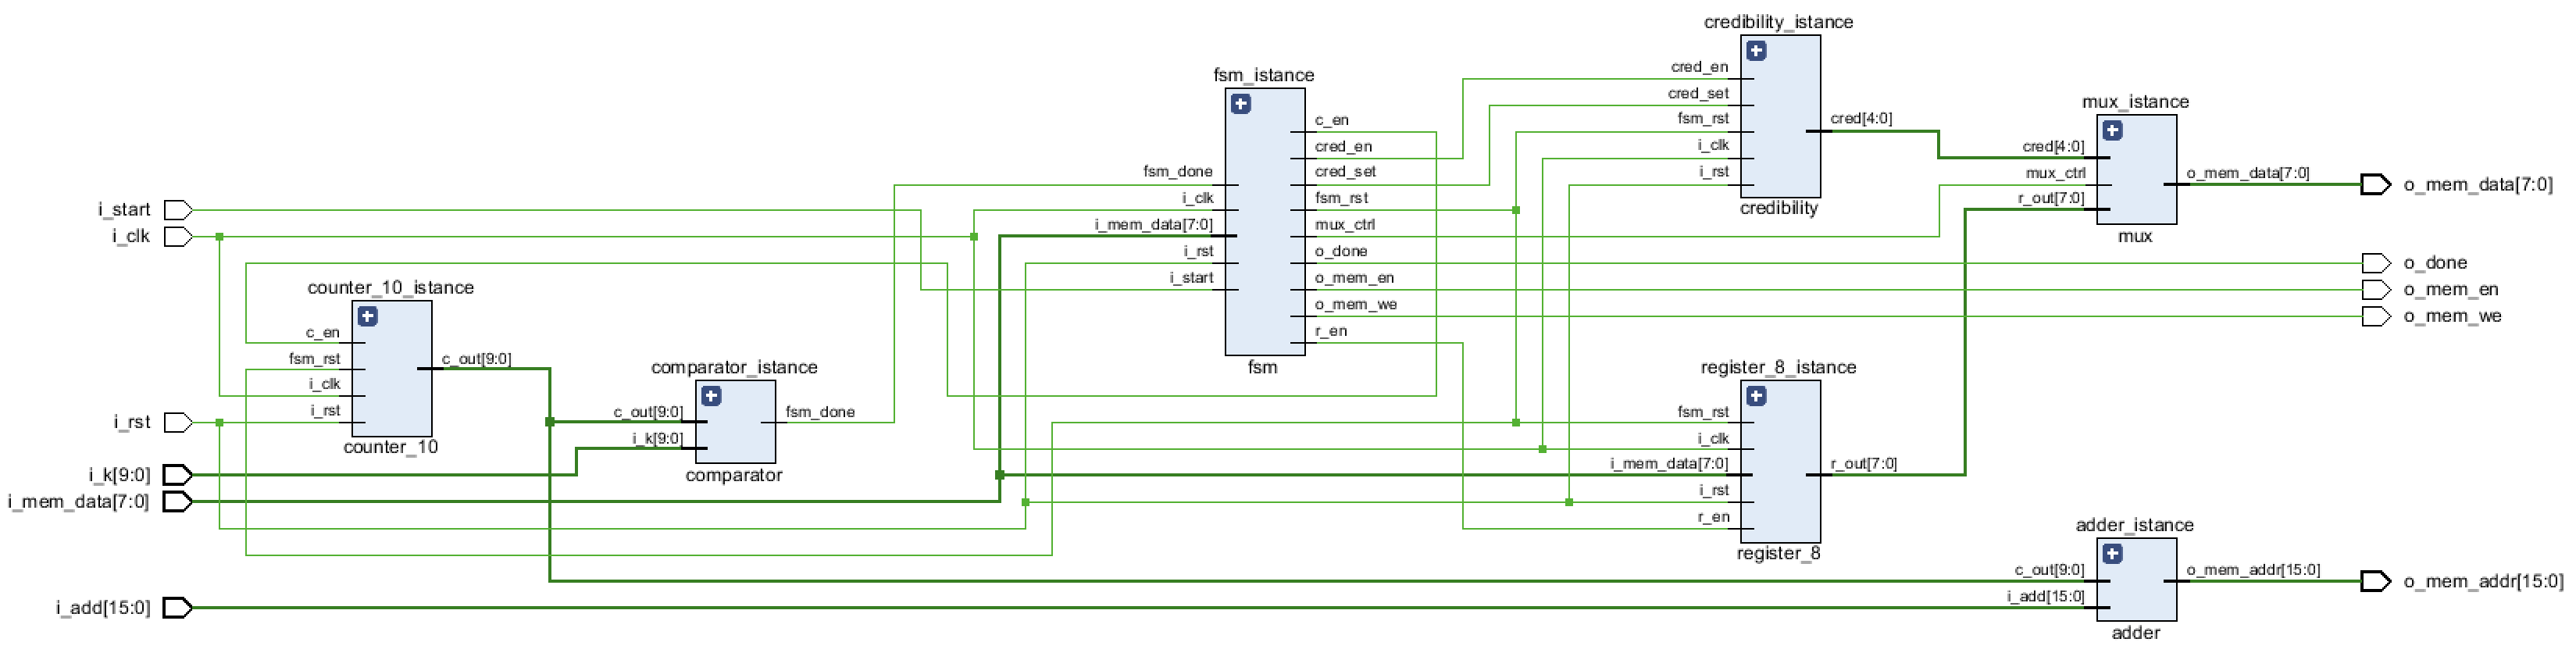
\includegraphics[width=1\textwidth]{figures/schematic.png}
    \caption{Design elaborato generato da Vivado}
    \label{fig:schematic}
\end{figure}

\subsubsection{Area utilizzata sulla FPGA}
Dal report di utilizzo otteniamo la seguente tabella dalla quale possiamo verificare l'assenza di latch indesiderati e la percentuale di utilizzo della FPGA utilizzata.
\begin{figure}[H]
    \centering
    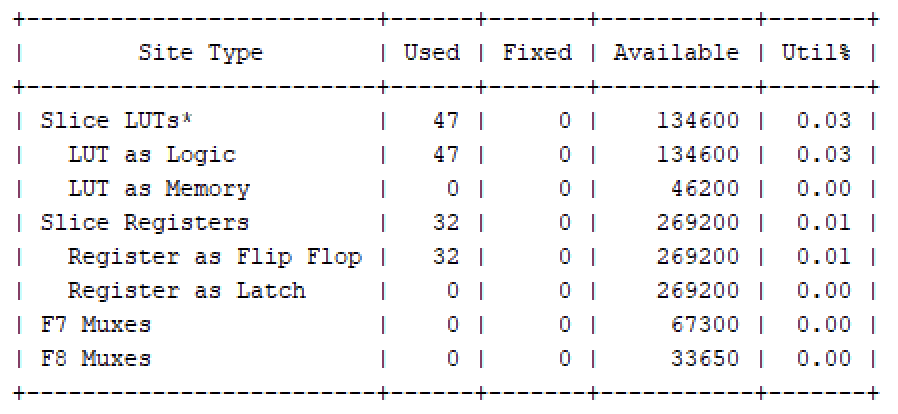
\includegraphics[width=0.75\textwidth]{figures/report_utilization.png}
    \caption{Report di utilizzo}
    \label{fig:report_utilization}
\end{figure}

\subsubsection{Frequenza di funzionamento}
Dal report temporale possiamo verificare che il componente soddisfa i requisiti di tempo. Considerando il periodo di clock $T_{clk}$ di $20 ns$, indicato nelle specifiche, si ottiene un  \textit{Worst Negative Slack} $WNS$ pari a $16.791ns$. Tramite un calcolo approssimativo è possibile ottenere la massima frequenza a cui può operare il componente.
\newline
Il minimo periodo utilizzabile risulta:
\begin{equation}
    T_{min} = T_{clk} - WNS = 20 ns - 16.791 ns = 3.209 ns
\end{equation}
Quindi si ottiene la massima frequenza di funzionamento:
\begin{equation}
    f_{max} = \frac{1}{T_{min}} = \frac{1}{3.209 ns} \approx 311.62 MHz.
\end{equation}
